\documentclass[]{beamer}
\usepackage[T1]{fontenc}
\usepackage[utf8]{inputenc}
\usepackage{lmodern}
\usepackage[italian]{babel}
\usepackage{mathrsfs}
\usepackage{cancel}

\title{L'induzione elettromagnetica}
\author{\texorpdfstring{Mattia Cozzi\newline\href{mailto:cozzimattia@gmail.com}{\texttt{cozzimattia@gmail.com}}}{Mattia Cozzi}}
\date{a.s.~2023/2024}

%\documentclass[handout]{beamer}     %usare questa classe per generare l'handout
%\usepackage{pgfpages}   %per mostrare più quadri nella stessa pagina
%\pgfpagesuselayout{4 on 1}[a4paper,border shrink=5mm,landscape]
\usetheme{Singapore}
%\useoutertheme[left]{sidebar} %elementi intorno alle diapositive
\setbeamercovered{dynamic} %modifica l'aspetto del testo grigetto delle diapositive future. Argomenti: invisible/transparent/dynamic
\usecolortheme{orchid}
%COLORE PRINCIPALE
\definecolor{marroncino}{RGB}{156, 26, 0} % UBC Blue (primary)
\setbeamercolor{structure}{fg=marroncino} % itemize, enumerate, etc

\theoremstyle{plain}
\newtheorem{teorema}{Teorema}

\usepackage{tikz}
\usepackage{circuitikz}


\usepackage{pgf,pgfplots,graphicx}
\usetikzlibrary{angles,quotes,arrows,shapes,decorations.markings}
\pgfplotsset{compat=1.15}
\usepgfplotslibrary{units,fillbetween} % to add units easily to axis
\tikzset{fleche/.style args={#1:#2}{postaction=decorate,decoration={name=markings,mark=at position #1 with {\arrow[#2,scale=2]{>}}},},}

\newcommand{\fem}{f_{em}}

\begin{document}

\begin{frame}
  \titlepage
\end{frame}





\begin{frame}
\frametitle{Contenuti}
\tableofcontents
\end{frame}


\section{Fenomeni induttivi}

\begin{frame}
  \frametitle{Magneti e correnti}
  Sappiamo che una corrente genera un campo magnetico (esperimento di \O rsted).\\~\\\pause
  \begin{block}{Domanda}
    Può un campo magnetico generare una corrente?
  \end{block}\pause
  ~\\Risposta positiva sarà data da Michael Faraday in Inghilterra e Joseph Henry negli Stati Uniti intorno al 1831.
\end{frame}







\begin{frame}
  \frametitle{Fenomeni induttivi (1)}
\begin{figure}
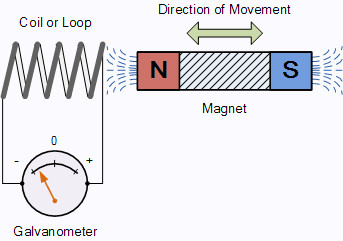
\includegraphics[width=.7\columnwidth]{img/induzione0.jpg}
\end{figure}
\end{frame}

\begin{frame}
  \frametitle{Fenomeni induttivi (2)}
\begin{figure}
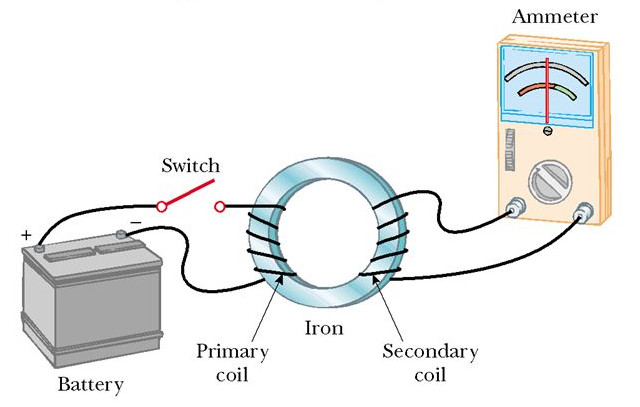
\includegraphics[width=.8\columnwidth]{img/induzione1.jpg}
\end{figure}
\end{frame}

\begin{frame}
  \frametitle{Fenomeni induttivi (3)}
\begin{figure}
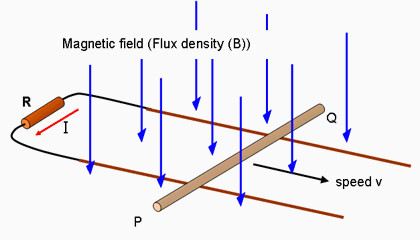
\includegraphics[width=.8\columnwidth]{img/induzione2.jpg}
\end{figure}
\end{frame}




\begin{frame}
  \frametitle{La variazione del flusso}
  Ricordando che:
\begin{center}
\colorbox{marroncino!30}{$ \Phi_S (\vec{B}) = \vec{B} \cdot \vec{S} = BS \cos\theta \quad [T \cdot m^2] = [Wb]$}
\end{center}\pause
possiamo affermare che  si ha una corrente indotta (causata da una forza elettromotrice indotta) ogniqualvolta si ha una variazione di flusso magnetico (causata da una variazione del campo, della superficie o dell'angolo che essi formano).\pause
\begin{block}{Causa della corrente indotta}
Si ha una corrente indotta quando varia il flusso del campo magnetico attraverso la superficie che ha per contorno il circuito indotto.
\end{block}
\end{frame}

\section{Faraday-Neumann-Lenz}


\begin{frame}
  \frametitle{Espressione matematica del legame tra $ fem_{ind} $ e flusso}
\begin{block}{Legge di Faraday-Neumann}
\[ fem_{ind} = - \frac{\Delta \Phi(\vec{B})}{\Delta t} \]\pause
Per la forza elettromotrice indotta istantanea:
\[ fem_{ist} = \lim_{\Delta t \rightarrow 0} \left( - \frac{\Delta \Phi(\vec{B})}{\Delta t} \right) = - \frac{d \Phi(\vec{B})}{d t} \]
\end{block}\pause
\begin{alertblock}{Attenzione}
La forza elettromotrice indotta istantanea è la derivata temporale del flusso del campo magnetico cambiata di segno.
\end{alertblock}
\end{frame}

\begin{frame}
  \frametitle{Il campo magnetico indotto}
  La variazione di flusso genera una corrente indotta.\pause

  ~
  
  La corrente indotta genera un campo magnetico ``indotto''.\pause

  ~
  
  Questo ``campo magnetico indotto'' può:
  \begin{itemize}
    \item rafforzare la variazione del campo esterno;\pause
    \item contrastare la variazione del campo esterno.\pause
  \end{itemize}
  \alert{La seconda opzione è l'unica possibile}: se la variazione venisse rafforzata, si genererebbe una corrente indotta ancora più intensa, che rafforzerebbe di nuovo la variazione, in un circolo infinito. Tutto ciò è in contrasto con il principio di conservazione dell'energia.
\end{frame}

\begin{frame}
  \frametitle{La legge di Lenz}
  \begin{block}{Legge di Lenz}
    Il verso della corrente indotta è sempre tale da \emph{opporsi alla variazione} di flusso che la genera.\pause
  \end{block}

  ~

  La legge di Lenz è espressa dal segno ``$ - $'' della legge di Faraday-Neumann (Legge di Faraday-Neumann-Lenz).
\end{frame}




\section{Corrente alternata}

\begin{frame}
  \frametitle{L'alternatore}
  
  \visible<1->{\begin{block}{Alternatore}
Un alternatore è un dispositivo che trasforma energia cinetica in energia elettrica.
\end{block}}
\visible<2->{È costituito da una spira che viene fatta ruotare con velocità angolare costante all'interno di un campo magnetico. La variazione di flusso magnetico genera una corrente indotta.
\begin{columns}
\begin{column}{0.3\textwidth}
\begin{figure}
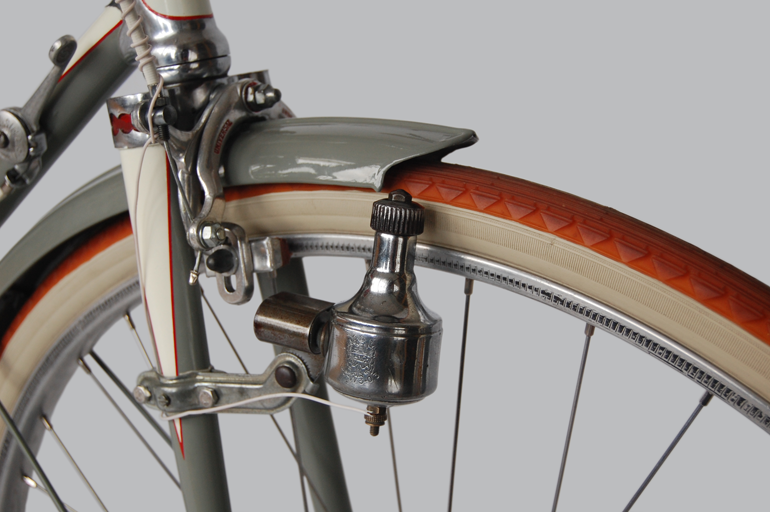
\includegraphics[width=\columnwidth]{img/alternatore1.png}
\end{figure}
\end{column}
\begin{column}{0.3\textwidth}
\begin{figure}
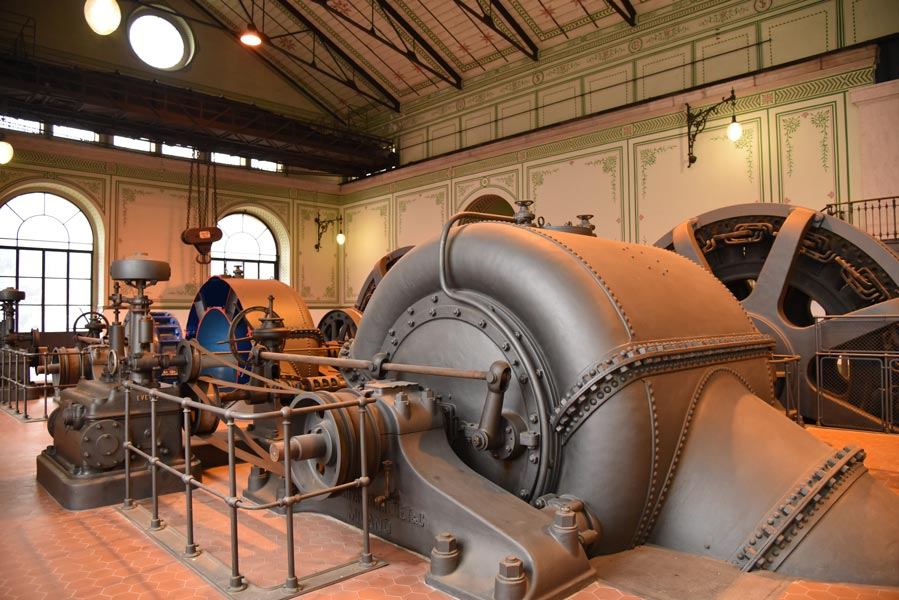
\includegraphics[width=\columnwidth]{img/alternatore2.jpg}
\end{figure}
\end{column}
\begin{column}{0.3\textwidth}
\begin{figure}\centering
\ctikzset{bipoles/length=1.5cm}
\begin{circuitikz}[scale=0.5]
\draw (0,0) to[vco, *-*] (4,0);
\end{circuitikz}
\end{figure}
\end{column}
\end{columns}}
\end{frame}



\begin{frame}
  \frametitle{Schema di un alternatore}
  \begin{figure}
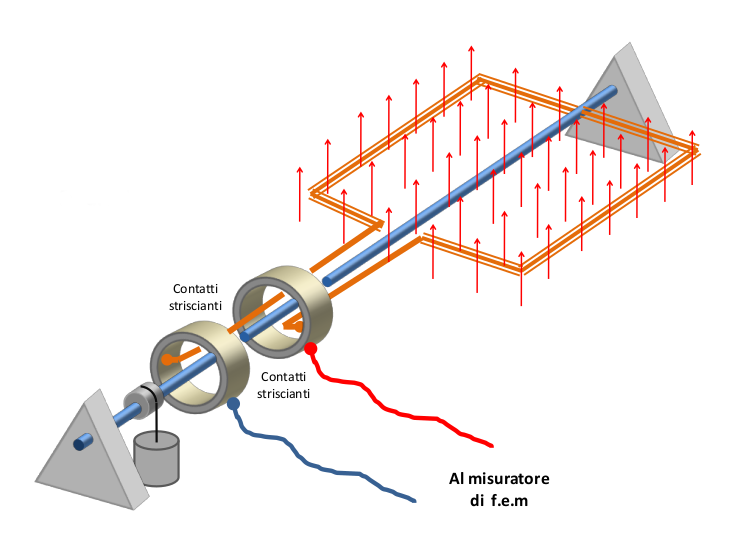
\includegraphics[width=0.8\columnwidth]{img/alternatore.png}
\end{figure}
\end{frame}


\begin{frame}
\frametitle{Grafico della corrente alternata}
\begin{figure}
  \begin{tikzpicture}[xscale=.4,yscale=1]
\node [left] at (0,1) {{\scriptsize $ i_0 $}};
\node [left] at (0,-1) {{\scriptsize $ - i_0 $}};
\node [above] at (1.5*pi,1) {{\scriptsize $ T = \dfrac{1}{f} $}};
\draw [->] (-4,0) -- (4*pi,0);
\node [below] at (4*pi,0) {{\scriptsize $ t \, [s] $}};
\node [left] at (0,2) {{\scriptsize $ i(t) \, [A] $}};
\draw [|<->|, dashed, thick] (.5*pi,1) -- (2.5*pi,1);
\draw [-, dotted] (.5*pi,1) -- (0*pi,1);
\draw [-, dotted] (0*pi,-1) -- (1.5*pi,-1);
\draw [->] (0,-2) -- (0,2);
\draw[smooth, red, thick, domain=-pi:3.5*pi] plot (\x, {sin(\x r)});
\end{tikzpicture}
\end{figure}

~

Valgono, come per ogni onda, le relazioni $ T = \dfrac{2 \pi}{\omega} $ e \colorbox{marroncino!30}{$ f = \dfrac{\omega}{2\pi} $}.\pause

~

In Europa $ f = 50 \, Hz $, mentre negli Stati Uniti $ f = 60 \, Hz $.
\end{frame}




\end{document}
